\chapter{Rapidly Deployable Hulls and On-demand Tunable Hydrodynamics with Shape Morphing Curved Crease Origami}\label{chapter-05}
Traditional hull fabrication relies on labour- and time-intensive methods to generate smooth, curved surfaces. These conventional methods often lead to hull surface topologies that are static in design with hydrodynamics aimed at handling a broad range of sea conditions but not optimized for any specific scenario. In this chapter, we introduce a method of rapidly fabricating planing hulls using the principles of curved-crease origami. Starting from a flat-folded state, the curved-crease origami hulls can be deployed to match traditional planing hull shapes like the VPS (deep-V, Planing hull with Straight face) and the GPPH (General Purpose Planing Hull). By extension of the ability to conform to a desired shape, we show that the curved-crease origami hulls can emulate desired hydrodynamic characteristics in still as well as wavy water conditions. Furthermore, we demonstrate the shape-morphing ability of curved-crease origami hulls, enabling them to switch between low and high deadrise configurations. This ability allows for on-demand tuning of the hull hydrodynamic performance. We present proof-of-concept origami hulls to demonstrate the practical feasibility of our method. Hulls fabricated using the curved-crease origami principles can adapt to different sea states, and their flat foldability and deployment facilitate easy transport and deployment for rapid response naval operations such as rescue missions and the launch of crewless aquatic vehicles. This work has been published as \href{https://doi.org/10.1016/j.jfluidstructs.2024.104176}{\textbf{Patil, H. Y.}, Maki, K. J., \& Filipov, E. T. (2024). Rapidly deployable hulls and on-demand tunable hydrodynamics with shape morphing curved crease origami. Journal of Fluids and Structures, 130, 104176}~\cite{patil2024ccohulls}.

\section{Introduction}\label{05-sec-origami-hull-intro}
Advanced boat-building and sailing technologies have existed since 6000 BCE~\cite{carter_boat_2006}. Despite the impressive technological strides in naval engineering over centuries, hull fabrication continues to be an enduring and intricate task. Hull fabrication relies on labor-intensive methods that involve connecting numerous flat sheets through bolting, riveting, or welding to form smooth, curved surfaces~\cite{paoli_fabrication_2012}. Achieving the necessary smooth curved surfaces also requires complex casting, milling, and molding procedures. Another challenge is that a significant portion of hull fabrication occurs in landlocked regions, necessitating the transportation of ship parts to coastal docks for assembly~\cite{bruce_ship_2021}. This transportation further extends the construction timeline and associated costs. These current hull fabrication techniques lead to designs with static surface topologies, resulting in hydrodynamics that are a compromise to accommodate a broad spectrum of sea conditions. Consequently, these hulls are not optimized for specific conditions, often leading to inefficient power consumption, poor maneuverability, and reduced passenger comfort and safety. For instance, crew members experience musculoskeletal pain and mental fatigue due to repeated exposure to vertical accelerations caused by the porpoising motion of vessels~\cite{bjorn_crew_2017}. These multifaceted challenges underscore the need to adopt innovative approaches in the shipbuilding industry, focusing on more versatile fabrication processes and improved adaptability in hull performance.

Origami, the age-old art of paper folding, presents a promising extension to the existing fabrication techniques used by the shipbuilding industry. In recent years, origami has transcended its traditional boundaries and found remarkable applications in engineering structures~\cite{meloni_engineering_2021}. One key characteristic of origami-inspired structures is their ability to transform flat sheets into complex, three-dimensional structures. This geometrically transformative process dynamically changes the properties of structures and the surrounding fluid media to meet multiple design objectives by varying the extent of folding, as shown by~\cite{chen_drag_2023} and~\cite{origami_flexiball_2023}. Origami-inspired designs embody several advantageous characteristics, each with unique applications. For instance, structures designed using origami principles can be rapidly deployed from compact configurations and easily reconfigured for various functions~\cite{zirbel_hanaflex_2015}. This reconfigurability has potential applications, such as creating stents for minimally invasive surgeries in biomedical engineering~\cite{kuribayashi_stent_2006} and improving the storage and deployment of satellites and solar arrays in space structures~\cite{bowen_starshade_2016}. Origami principles are also scale-independent~\cite{dudte_scale_2016}, making them applicable to structures ranging from deployable stadium canopies to micro-scale sensors. Additionally, the active folding capability enables these structures to change form on demand, increasing their adaptability to various loads and conditions \textemdash{} a strategy often employed by biological organisms to survive in strong winds or water currents~\cite{harder_reconfiguration_2004}. Thus, incorporating origami principles into ship hull design offers benefits such as flat foldability, efficient storage and transport, and rapid deployment.

While traditional origami surfaces such as Miura-ori~\cite{k_science_2008} are characterized by rough and angular profiles, curved-creasing \textemdash{} a subset of origami, provides a groundbreaking approach to fabricating hull-type structures in naval engineering. Research by~\cite{erik_demaine_curved_2011} demonstrates that folding a sheet of material along arbitrary non-intersecting curved creases enables rapid and easy fabrication of smooth curved surfaces. Curved-crease origami preserves the inherent merits of conventional origami techniques while offering numerous benefits suited for hull fabrication. For instance, curved creasing grants precise control over surface topologies by tuning the crease geometry and extent of actuation. Furthermore, it enables the fabrication of complex 3-D shapes that embody benefits such as reduced joint complexity, increased global stiffness, and improved resistance to buckling~\cite{woodruff_curved_2021}.

Motivated by the potential of curved-crease origami principles, this chapter presents an approach for fabricating planing hulls. Planing hulls commonly feature a V-shaped bottom and a transom stern design, which generates hydrodynamic lift to support the hull weight and enable high-speed travel. As a result, these hulls are widely used for applications such as Coast Guard boats, rescue vessels, and ocean racers~\cite{savitsky_planing_1985}. \cite{tavakoli_review_2024} provides a detailed review of the topology and hydrodynamics of planing hulls. The inherent geometry of planing hulls (see Section~\ref{05-sec-geometry-curved-folding}) makes them an ideal candidate for incorporating curved-crease origami-based fabrication techniques. Thus, as a first step towards curved-crease origami-based hulls, we limit the scope of our exploration to idealized planing hulls. While we agree that extending origami principles to general hull forms poses several challenges at this stage, it still holds significant potential for curved surface fabrication and will be explored separately in the future.

By leveraging the principles of origami, we demonstrate the capability to reproduce a predetermined target planing hull shape with precision. This capability enables the emulation of a desired hydrodynamic behavior and embodies the fabrication efficiency inherent to curved crease origami. Furthermore, through the strategic utilization of active folding in curved-crease origami hulls, we illustrate their ability to undergo a characteristic shape change in real-time. This shape morphing behavior enables on-demand tunability of hydrodynamic properties and renders them applicable across a wide variety of sea conditions. Hulls fabricated using the proposed methods can adapt to any sea state, and their flat foldability and rapid deployment will facilitate easy transport and deployment for naval operations such as covert rescue missions and the launch of crewless decoy marine vehicles. These vehicles will also improve sea-keeping performance, power efficiency, maneuverability, and passenger comfort, making them suitable for civilian recreational use.

The remainder of the chapter is organized as follows. Section~\ref{05-sec-geometry-curved-folding} reviews standard planing hull geometries and curved folding procedures. The subsections discuss the planing behavior and typical geometric features of a planing hull, the development of a curved-origami crease pattern for the planing hull, an overview of the numerical model for curved-origami folding, and geometric parameter optimization to match curved-origami hulls to their target shape. Next, Section~\ref{05-sec-hydrodynamic-analysis} explores the hydrodynamic analyses and performance evaluation of curved origami planing hulls against target hull shapes. The core findings of this chapter, including the on-demand shape morphing capabilities of curved-origami hulls and tunable hydrodynamic characteristics for a wide range of sea conditions, are presented in Section~\ref{05-sec-tunable-hydrodynamics}. A discussion on the scalability of origami hulls with an emphasis on curvature analysis for various construction materials is presented in Section~\ref{05-sec-physical-implementation}. Finally, concluding remarks summarizing the key contributions are included in Section~\ref{05-sec-hull-conclusion}.

\section{Geometry and Curved Folding}\label{05-sec-geometry-curved-folding}    

\subsection{Planing Hull Geometry}\label{05-subsec-planing-geometry}
In a state of rest, buoyant forces are responsible for bearing the weight of a floating hull. Buoyancy is also crucial at lower speed since the hull stays afloat by displacing a volume of water. However, as the speed increases, hydrodynamic lift becomes dominant over the buoyant force and supports the weight of the hull. This hydrodynamic lift allows a planing hull to rise and glide on the water surface.

A typical planing hull has distinct geometric features that enable it to generate hydrodynamic lift. These geometric features of a planing hull (some illustrated in Fig.~\ref{fig-planing-geometry}\,(a)) can be defined as follows: \mbox{(\textit{i}\hspace{.5pt})} \textit{Bow}: the foremost part of the hull; \mbox{(\textit{ii}\hspace{.5pt})} \textit{Chine}: line along which a sharp change in the angle of cross-section occurs; \mbox{(\textit{iii}\hspace{.5pt})} \textit{Deadrise}: the angle between the bottom of the hull and horizontal surface; \mbox{(\textit{iv}\hspace{.5pt})} \textit{Draft}: the distance between the waterline and the deepest part of the boat in steady state; \mbox{(\textit{v}\hspace{.5pt})} \textit{Hull Bottom}: bottom surface of the hull (also called the planing surface); \mbox{(\textit{vi}\hspace{.5pt})} \textit{Keel}: bottom-most longitudinal structural element of a hull; \mbox{(\textit{vii}\hspace{.5pt})} \textit{Sheer line}: the uppermost edge of the hull; \mbox{(\textit{viii}\hspace{.5pt})} \textit{Stern}: the aftmost part of the hull; \mbox{(\textit{ix}\hspace{.5pt})} \textit{Transom}: the flat board extending from the keel to the deck at the stern; \mbox{(\textit{x}\hspace{.5pt})} \textit{Trim}: the angle between the horizontal surface and the line connecting the forward and the aft draft; and \mbox{(\textit{xi}\hspace{.5pt})} \textit{Waterline}: the level water reaches on the hull's side. In some cases, the hull has a parallel section and can be divided into two parts longitudinally, namely the prismatic and non-prismatic sections. The prismatic section often forms the middle to aft half of the hull where the keel and chine lines are parallel. On the other hand, the non-prismatic section forms the front portion of the hull where the keel and chine lines are no longer parallel.

It is important to note that the planing hulls discussed in this chapter are hard-chined vessels, which means that the hull exhibits a distinct change of angle along the chine, where the bottom surface meets the sides of the boat. Additionally, these planing hulls feature a typical V-shaped bow with straight surfaces instead of an axe, bulbous, parabolic, or flared bow.

\begin{figure}[!htbp]
  \centering
  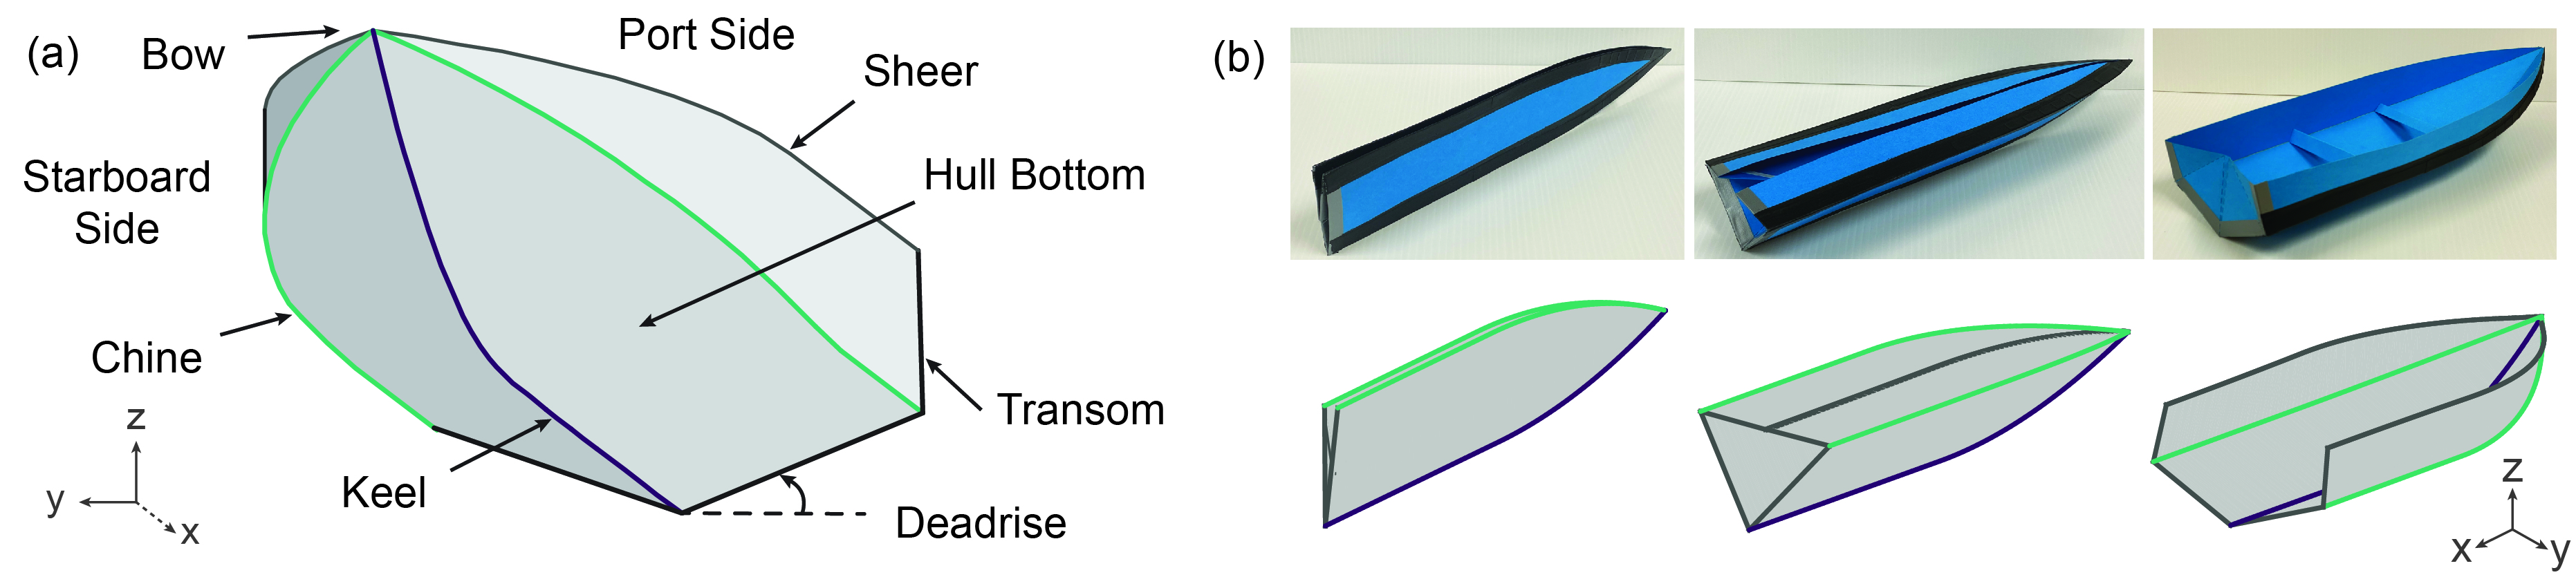
\includegraphics[width=\textwidth]{01-figures/05-01-geometry-and-hull-folding.jpg}
  \caption{(a) Geometric features of a typical planing hull: specifically a deep V-shape, Planing hull with a Straight planing surface (VPS); (b) Sequential deployment of curved-crease origami hull designed to match the shape of a VPS hull: paper model (top) compared with Bar and Hinge simulation (bottom). A transom is not included in the simulation.}\label{fig-planing-geometry}
\end{figure}

The curved-crease origami-inspired planing hulls offer a method to change some of the aforementioned geometric features that directly affect the hull's planing ability, stability, ride comfort, maneuverability, and power efficiency. Throughout its deployment, the curved crease origami hulls can vary the deadrise, hull length, topology of the curved planing surface, and beam length. The deployment process from a flat-folded to a deployed-hull state is shown in Fig.~\ref{fig-planing-geometry}\,(b) for both a 20-inch long paper prototype and for a corresponding Bar and Hinge simulation (discussed in the following section). The planing hull design, obtained using the bar and hinge model, is presented here without the transom to reveal distinctive features of the hull, including the chine, keel, and profile of the planing surface. However, the transom can be incorporated into the model, akin to the paper prototype shown in Fig.~\ref{fig-planing-geometry}\,(b).

\subsection{Crease Geometry and Bar and Hinge Model for Curved Folding}\label{05-subsec-crease-bnh}
A curved crease pattern presented in Fig.~\ref{fig-crease-bnh}\,(a) is developed to match the VPS hull designed by~\cite{kim_design_2013}. VPS stands for deep V-shape, Planing hull with a Straight planing surface, and resembles the shape illustrated in Fig.~\ref{fig-planing-geometry}\,(a). This crease pattern unfolds into a 3D shape with all the geometric features of a typical planing hull. The geometric parameters used to define this crease pattern are: \mbox{(\textit{i}\hspace{.5pt})} width of the hull's bottom surface between the chine and the keel, \(H\); \mbox{(\textit{ii}\hspace{.5pt})} height of the tip, \(h_{\textrm{tip}}\); \mbox{(\textit{iii}\hspace{.5pt})} overall length of the crease pattern, \(L_{OA}\); \mbox{(\textit{iv}\hspace{.5pt})} length of the prismatic part of the chine, \(L_{P}^{c}\); \mbox{(\textit{v}\hspace{.5pt})} length of the non-prismatic part of the chine, \(L_{N}^{c}\); \mbox{(\textit{vi}\hspace{.5pt})} length of the prismatic part of the keel, \(L_{P}^{k}\); and \mbox{(\textit{vii}\hspace{.5pt})} length of the non-prismatic part of the keel, \(L_{N}^{k}\). The curved portions (non-prismatic section) of the chine and the keel curves are parabolic and denoted by \(y_c\) in Eq.~\ref{eq-chine-curve} and \(y_k\) in Eq.~\ref{eq-keel-curve}, respectively. For a given overall length of the crease pattern, the length of the non-prismatic section for the chine and keel curves are denoted by \(L_N^c\) in Eq.~\ref{eq-np-chine} and \(L_N^k\) in Eq.~\ref{eq-np-keel}, respectively. These quantities can be computed as:
\begin{flalign}
  \quad L_{N}^{c} & = L_{OA} - L_{P}^{c}~,&\label{eq-np-chine}\\
  \quad L_{N}^{k} & = L_{OA} - L_{P}^{k}~,&\label{eq-np-keel}\\
  \quad y_{k} & = \left[\frac{h_{\textrm{tip}}}{{L_{N}^{k}}^2}\right]\times\left(x-L_{P}^{k}\right)^2~,&\label{eq-keel-curve}\\
  \quad y_{c} & = \left[\frac{h_{\textrm{tip}}-H}{{L_{N}^{c}}^2}\right]\times\left(x-L_{P}^{c}\right)^2 + H~.&\label{eq-chine-curve}
\end{flalign}

\begin{figure}[!htbp]
  \centering
  \includegraphics[width=\textwidth]{01-figures/05-02-crease-pattern-and-bar-hinge.jpg}
  \caption{(a) Geometric parameters defining the curved crease pattern for a planing hull shape; (b) Folded curved-crease origami hull shape viewed from starboard side; (c) Flat, intermediate, and fully folded (clockwise from top) curved-crease origami hull shape viewed from the Transom (also known as Stern) side; and (d) Decomposition of the Bar and Hinge model into its components: in-plane bars, bending hinges, and folding hinges.}\label{fig-crease-bnh}
\end{figure}

The curved folding simulation of the origami crease pattern into a planing hull shape is accomplished through the Bar and Hinge model developed by~\cite{woodruff_bar_2020}. This model offers a simplified numerical approach that effectively simulates the fundamental behaviours of curved origami folding by employing three distinct elements, as illustrated in Fig.~\ref{fig-crease-bnh}. These elements can be described as follows: \mbox{(\textit{i}\hspace{.5pt})} three-dimensional truss elements, or bars, that capture in-plane stretching and shearing of the sheet; \mbox{(\textit{ii}\hspace{.5pt})} rotational springs, or hinges, that capture the out-of-plane bending of the sheet by consolidating bending into discrete rotations along the bar lengths; and \mbox{(\textit{iii}\hspace{.5pt})} another set of hinges that capture the rotations at the creases or fold lines.

The crease pattern is meshed using a combination of the three elements, where the stiffness of each element is determined based on material properties, sheet thickness, and mesh size. Despite the inherent geometric nonlinearity involved in the folding process, the model achieves convergence within a short time frame (less than 10 seconds). This rapid convergence is due to the relatively low number of elements in the Bar and Hinge model compared to finite element methods. Consequently, this rapid simulation enables efficient analysis of curved origami structures, facilitating subsequent shape-matching and optimization processes.

\subsection{Shape Matching and Optimization}\label{05-subsec-shape-matching}
The geometric design parameters presented in Fig.~\ref{fig-crease-bnh}\,(a) can be varied and optimized such that the curved crease origami (CCO) hull shape will match the desired target shape. The matching of CCO hull with target hull shapes is significant for two reasons. Firstly, it enables the reproduction of specific hydrodynamic characteristics by replicating the target shape. Secondly, it facilitates the integration of origami-based design principles in conventional hull design, thereby unlocking the potential to design on-demand shape morphing hulls with tunable hydrodynamics. This section will explore two design variations of the CCO hulls, CCO\(^\textrm{VPS}\) and CCO\(^\textrm{GPPH}\), and compare their shapes with those of the VPS and the General Purpose Planing Hull (GPPH) shapes, respectively.

\begin{figure}[!htbp]
  \centering
  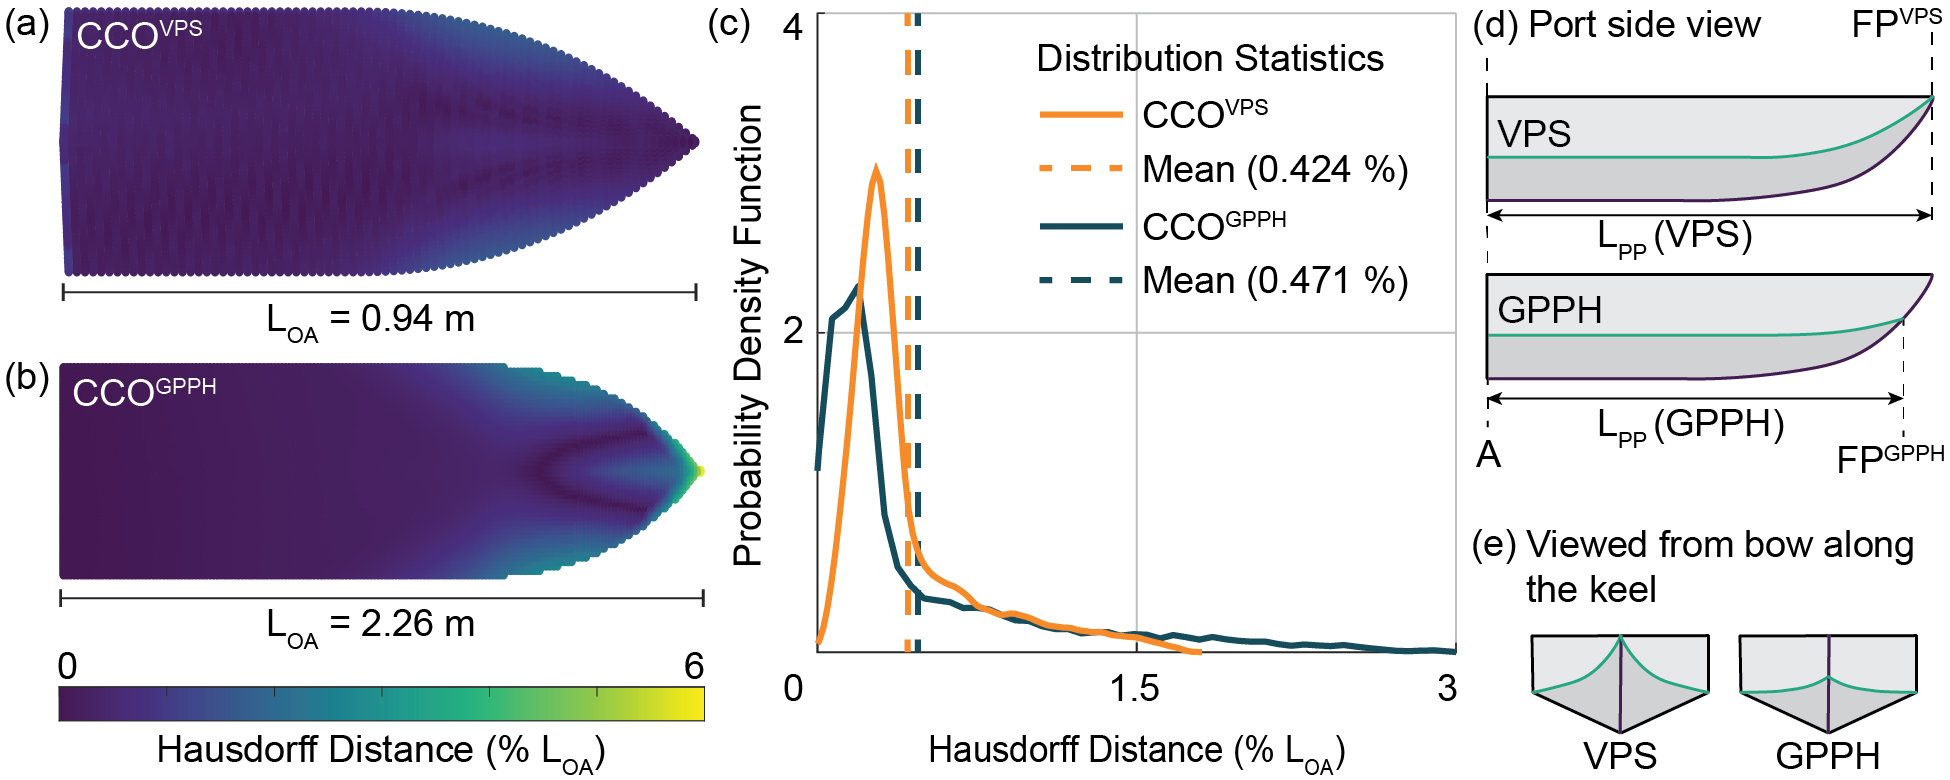
\includegraphics[width=\textwidth]{01-figures/05-03-hausdorff-shape-matching-optimization.jpg}
  \caption{Color heat map showing the Hausdorff distance as a percentage of the overall hull length (\(L_{OA}\)) for the planing surface of two different CCO hull designs compared with: (a) 0.94 m long VPS hull and (b) 2.26 m long GPPH, respectively; (c) Hausdorff distance distribution statistics for CCO hull designs' planing surface compared with corresponding VPS and GPPH designs; (d) Port side view depicting the location of forward perpendicular (FP), aft perpendicular (AP) and the length between the two perpendiculars (\(L_{PP}\)); and (e) Bow view when looked along the keel of the VPS and GPPH showing the difference in the chine and keel configuration.}\label{fig-shape-matching}
\end{figure}

The quantification of dissimilarity between a CCO hull shape and a target shape is performed using a parameter called the Hausdorff distance, \(d_H\). By definition, the Hausdorff distance represents the maximum distance between any point in one set and the closest point in the other set in three-dimensional space, indicating the largest discrepancy between the two point sets. Hence, smaller Hausdorff distances between two sets (two shapes in this case) indicate a closer match. To ensure consistency in comparing the two different design variants of the CCO hulls with their target shapes, we will represent the Hausdorff distance as the percentage of the overall length, \(L_{OA}\) of the hull's planing surface. We specifically emphasize comparing the planing surface because its interaction with water is the predominant factor that influences the hydrodynamic behavior of the hull.

The planing surfaces of CCO\(^\textrm{VPS}\) and VPS hulls are populated with approximately 5000 points, and the Hausdorff distance for each point on the CCO\(^\textrm{VPS}\) hull is computed with respect to the VPS hull (Fig.~\ref{fig-shape-matching}\,(a)). As the folded shape of the CCO\(^\textrm{VPS}\) hull is influenced by the geometric parameters of the curved-crease pattern, a simple optimization problem is formulated to find optimal values that minimize the Hausdorff distance between the two hulls. The objective of this problem is to minimize the mean Hausdorff distance between the two hulls, considering the following design variables: \mbox{(\textit{i}\hspace{.5pt})} overall length of crease pattern (\(L_{OA}\)), \mbox{(\textit{ii}\hspace{.5pt})} width of the planing panel (\(H\)), \mbox{(\textit{iii}\hspace{.5pt})} tip height (\(h_\textrm{tip}\)), \mbox{(\textit{iv}\hspace{.5pt})} length of the prismatic part of chine (\(L_P^c\)), \mbox{(\textit{v}\hspace{.5pt})} length of the prismatic part of the keel (\(L_P^k\)), and  \mbox{(\textit{vi}\hspace{.5pt})} deadrise of the hull. The optimizer successfully achieves a mean Hausdorff distance of 0.424\% and a maximum Hausdorff distance of under 2\% of the overall length of the hull, indicating an excellent match between the two shapes. This method enables on-demand replication of hull shapes using curved-crease origami principles for innovative hull design and hydrodynamic optimization.

A similar shape-matching procedure is performed for the CCO\(^\textrm{GPPH}\) and the GPPH hulls with approximately 7500 points. In this case, the mean Hausdorff distance is observed to be 0.471\%, and the maximum Hausdorff distance is under 6\% of the overall GPPH length. The larger Hausdorff distances compared to the previous case, particularly towards the bow of the hull (see Fig.~\ref{fig-shape-matching}\,(b)), can be explained by the difference in the keel extension of the hull designs. As illustrated in Fig.~\ref{fig-shape-matching}\,(d) and (e), the keel line of the GPPH extends beyond the chine. Meanwhile, the chine and keel lines of the VPS and both CCO hull designs terminate at the same point on the hull's bow. This difference in keel extension leads to a dissimilar bow shape in the GPPH design compared to the VPS and both CCO hull designs, thus explaining the higher Hausdorff distances.

Despite the minor dissimilarities observed near the bow of the hull in the cases of the VPS and GPPH, the CCO hulls achieve a close match over the prismatic section of the planing surface. The mean Hausdorff distance for the prismatic section of VPS and GPPH equivalent CCO hulls is observed to be 0.258\% and 0.281\% of the overall length, respectively.  Furthermore, the distribution of Hausdorff distances shown in Fig.~\ref{fig-shape-matching}\,(c) indicates that the mean Hausdorff distance is less than 0.5\% of the overall length for most parts of the planing surface that would interact with water. This similarity in shape and deadrise ensures that the CCO hull can potentially exhibit hydrodynamic characteristics comparable to those of the conventional VPS and GPPH hull designs. Detailed findings related to the hydrodynamic properties and the comparison between the CCO hulls, VPS, and GPPH are presented and discussed in the subsequent sections.

\section{Hydrodynamic Performance Evaluation of Curved-crease Origami Hulls}\label{05-sec-hydrodynamic-analysis}
The ability of curved-crease origami (CCO) hulls to align congruently with target hull shapes motivates a comparative investigation to evaluate whether their hydrodynamic characteristics also match those of the conventional hulls. This section compares the hydrodynamic performance of the two distinct CCO hull variants, CCO\(^\textrm{VPS}\) and CCO\(^\textrm{GPPH}\) as introduced in Section~\ref{05-subsec-shape-matching}, with their corresponding target hull forms, namely the VPS and the GPPH. The hydrodynamic evaluation for all four hull geometries is facilitated by the Powersea tool and encompasses the simulation of hull motion in both still and wavy water (head sea) conditions. Powersea's underlying theory, assumptions and limitations can be found in Appendix~\ref{03-appendix-powersea}. The geometric and physical characteristics of the hulls passed as input to Powersea can be found in Table~\ref{tab-cco-hull-geom}.
\begin{table}[h!]
  \caption{Geometric and physical characteristics of the hulls for hydrodynamic simulations}
  \vspace{-1.5em}
  \begin{center}
	\begin{tabularx}{\textwidth}{ >{\raggedright\arraybackslash}X >{\centering\arraybackslash}m{0.4in} >{\centering\arraybackslash}m{0.4in} >{\centering\arraybackslash}m{0.6in} >{\centering\arraybackslash}m{0.6in} >{\centering\arraybackslash}m{0.6in} >{\centering\arraybackslash}m{0.7in} >{\centering\arraybackslash}m{0.5in} }
  	\hline
  	\multirow{2}{3.5in}{\textbf{Hull geometry}} & \textbf{L$_{OA}$} & \textbf{L$_{PP}$} & \textbf{LCG } & \textbf{VCG} & \textbf{K$_{yy}$} & \textbf{Weight} & \textbf{B}\\
  	& (m) & (m) & (\% L$_{OA}$) & (m) & (\% L$_{OA}$) & (N) & (m)\\
  	\hline
    \noalign{\vskip 3pt}
  	CCO\(^\textrm{VPS}\) & 0.94 & 0.92 & 62 & 0.056 & 25 & 65 & 0.312\\  
  	VPS & 0.94 & 0.92 & 62 & 0.056 & 25 & 65 & 0.308\\
  	CCO\(^\textrm{GPPH}\) & 2.26 & 2.26 & 62 & 0.097 & 25 & 995.51 & 0.583\\
  	GPPH & 2.26 & 2.23 & 62\small{(\%\,\(L_{PP}\))} & 0.097 & 25\small{(\%\,\(L_{PP}\))} & 995.51 & 0.615\\
  	\hline  
	\end{tabularx}
  \end{center}\label{tab-cco-hull-geom}
  \vspace{-1em}
\end{table}

The still water simulations for all four hull shapes are conducted for various constant speed cases. For the VPS and CCO\(^\textrm{VPS}\) hulls, these speeds range from 2 to 15.5 m/s. For GPPH and CCO\(^\textrm{GPPH}\) hulls these speeds range from 2.5 to 20.5 m/s. The speeds correspond to beam Froude numbers, \(F_B\) ranging from 1 to 9 for each of the four hull geometries. The beam Froude number is calculated as \(F_B = U / \sqrt{g \times B}\), where \(U\) is the speed, \(g\) is the acceleration due to gravity and \(B\) is the beam width (distance between the two keels at transom). Other simulation parameters adhered to the default values specified by Powersea, and the hydrodynamic characteristics are shown in Fig.~\ref{fig-calm-cco-eval}. The hydrodynamic characteristics include: \mbox{(\textit{i}\hspace{.5pt})} friction drag experienced by the hull due to the shearing of the fluid boundary layer normalized by the hull weight, \mbox{(\textit{ii}\hspace{.5pt})} total resistance \textemdash{} a combination of friction drag, viscous pressure drag and wave making resistance, normalized by the hull weight, \mbox{(\textit{iii}\hspace{.5pt})} Rise of Center of Gravity (CG) \textemdash{} heave displacement relative to at-rest position normalized by the beam width, and \mbox{(\textit{iv}\hspace{.5pt})} trim \textemdash{} running angle of the hull about its lateral axis as it makes way in the water. While the friction drag, rise of CG, and pitch data are generated by Powersea, the weight normalized total resistance, \(R_T / W\), is calculated as follows:
\begin{flalign}
  \quad \frac{R_T}{W} & = \tan{(\eta_5)} + \frac{D}{W}\times\frac{1}{\cos{(\eta_5)}}~,&\label{eq-friction-drag}
\end{flalign}
where \(D\) is the friction drag, \(W\) is the weight of the hull, and \(\eta_5\) is the pitch (trim angle)~\cite{doctors_hydrodynamics_1985}. It is important to note that the total resistance does not include whisker spray drag.

\begin{figure}[!htbp]
  \centering
  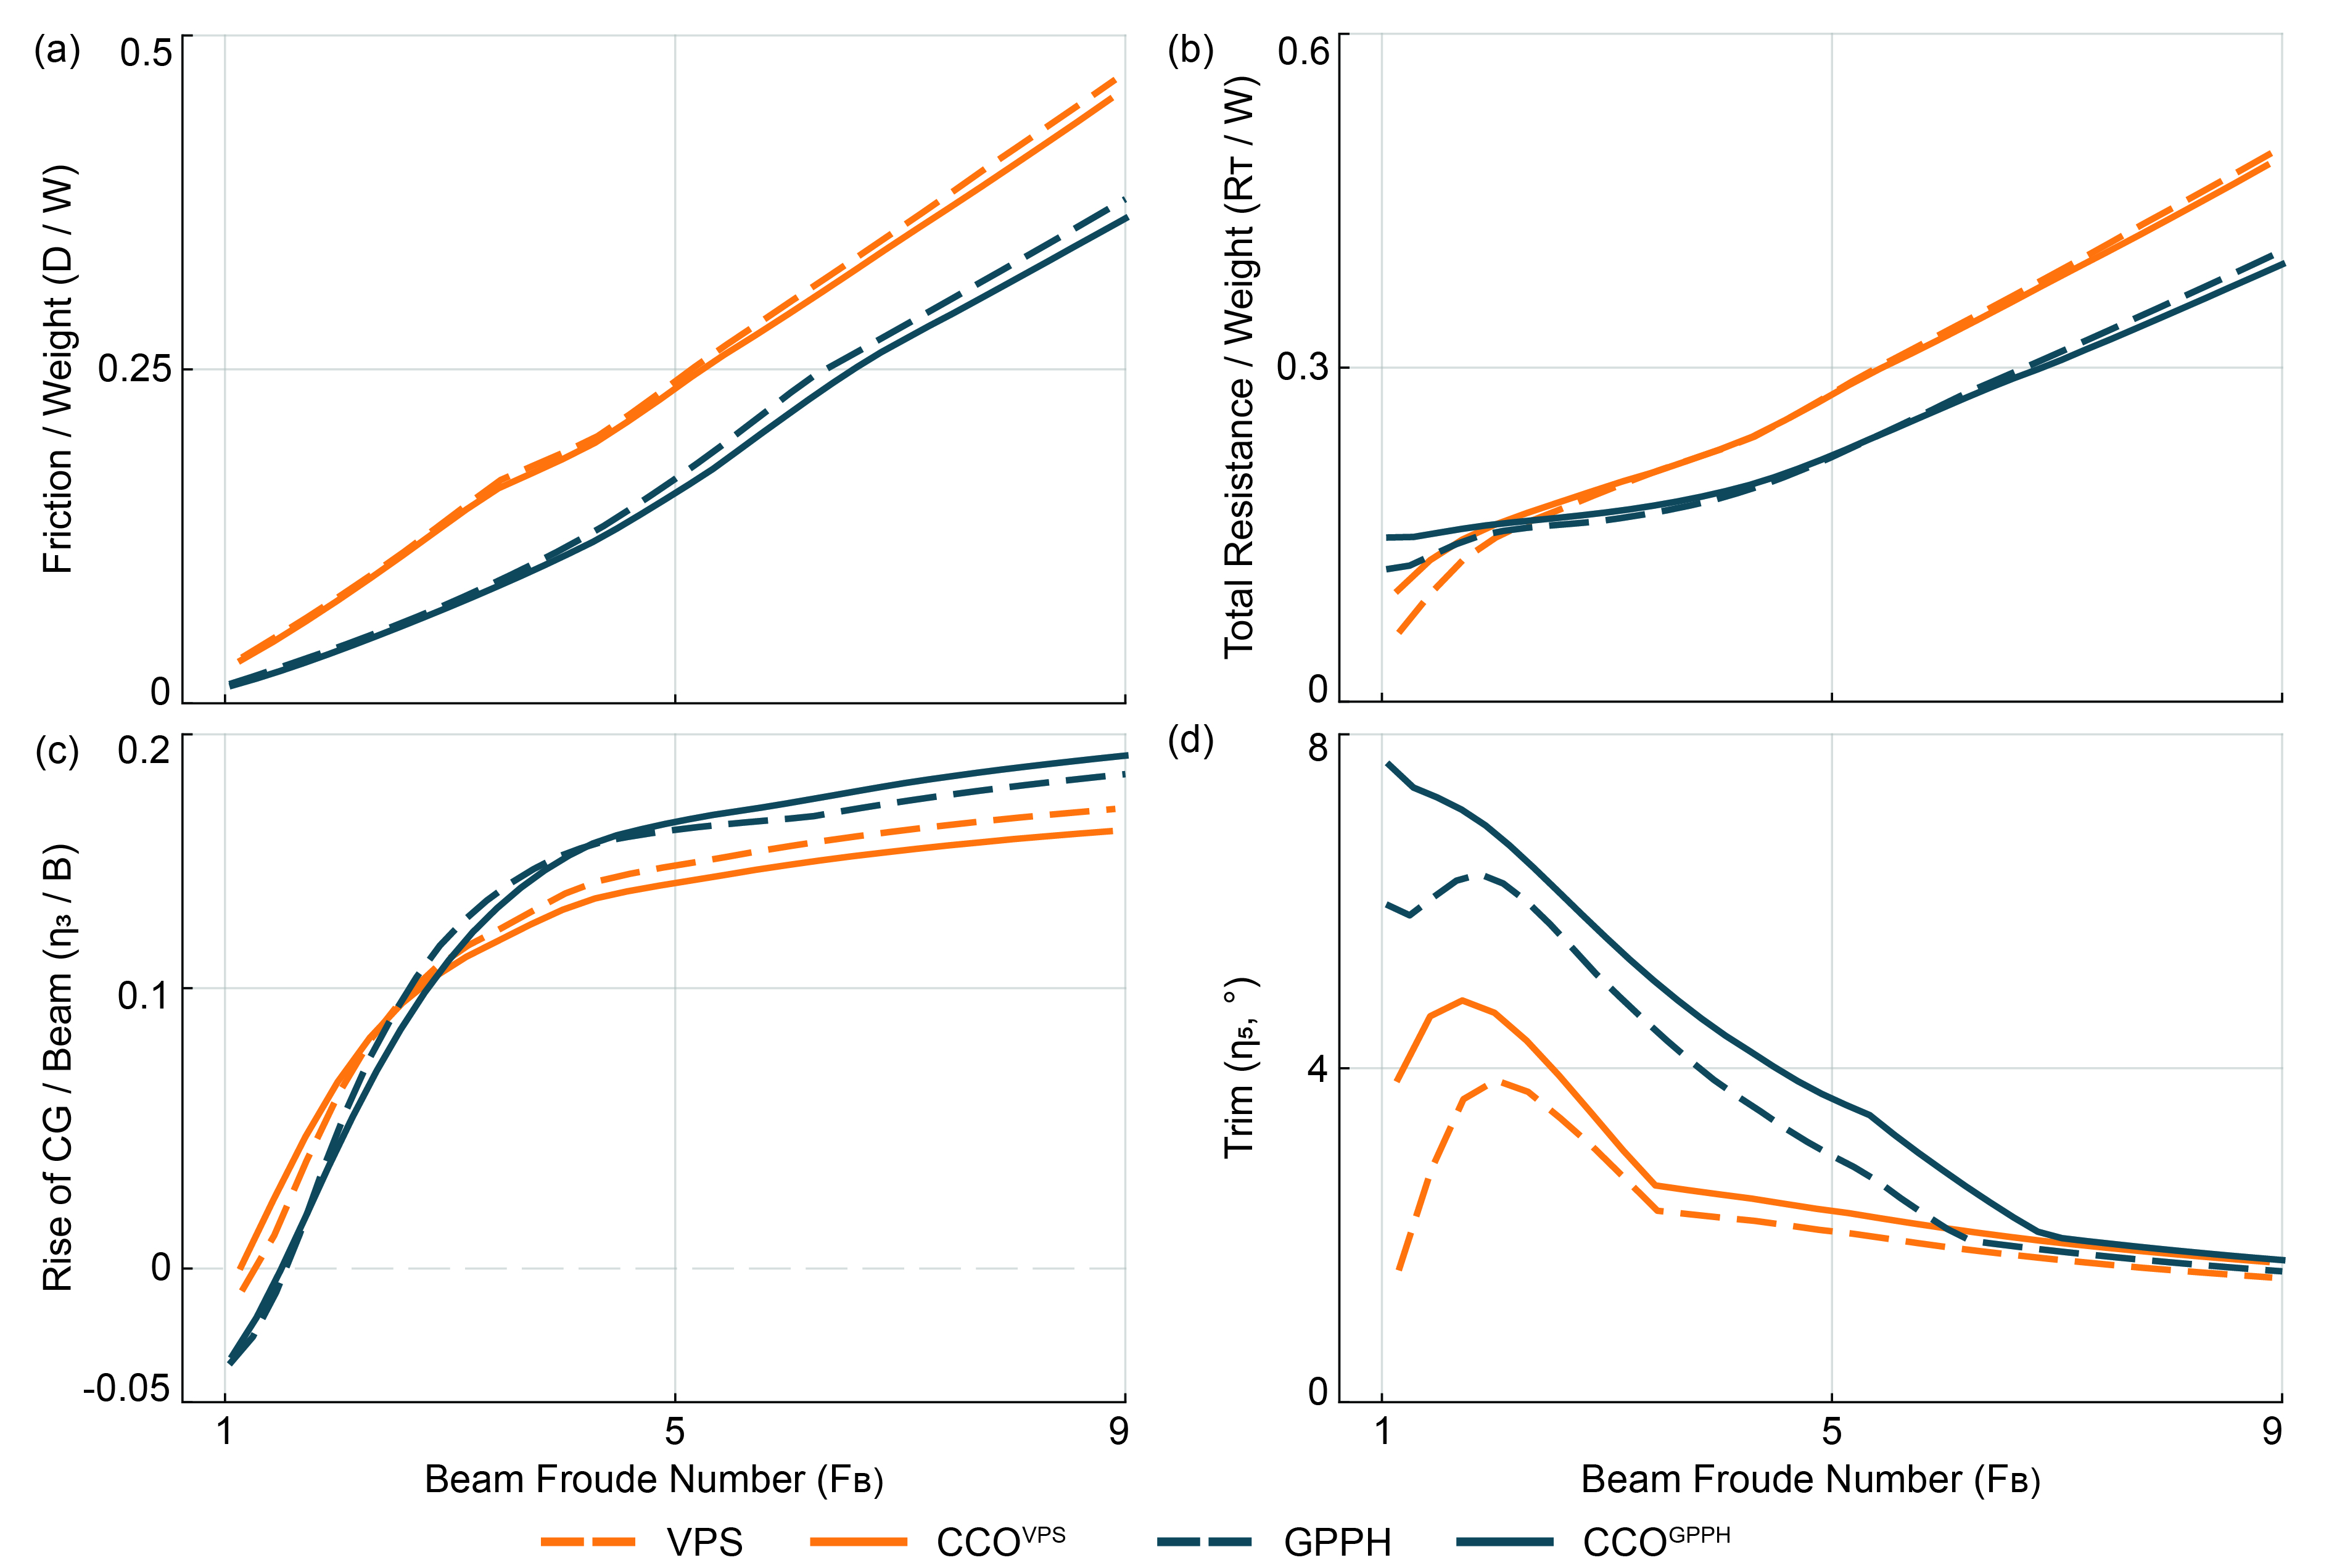
\includegraphics[width=\textwidth]{01-figures/05-04-calm-cco-eval.jpg}
  \caption{Comparison of VPS and GPPH hydrodynamics with their CCO counterparts in calm water: (a) Weight normalized friction drag; (b) Weight normalized total resistance; (c) Beam normalized rise of CG; and (d) Trim angle (positive bow up)}\label{fig-calm-cco-eval}
\end{figure}

It is essential to note that the comparative analysis of CCO hulls with counterparts GPPH and VPS hulls reveals a consistent trend across various hydrodynamic characteristics. Both friction drag in Fig.~\ref{fig-calm-cco-eval}\,(a) and total resistance in Fig.~\ref{fig-calm-cco-eval}\,(b) exhibit a monotonically increasing trend as the planing speed increases. Additionally, the hull tends to rise on the water surface with an increase in planing speed, as evidenced by the rise in CG illustrated in Fig.~\ref{fig-calm-cco-eval}\,(c). Contrarily, the trim angle of the hull diminishes with an increase in the planing speed, as indicated in Fig.~\ref{fig-calm-cco-eval}\,(d). However, it is also imperative to acknowledge a slight disparity in the trim angle of the CCO hulls and their GPPH and VPS counterparts. The following reasons can explain this disparity. First, despite exhibiting a close match, the CCO hulls are not identical in shape to their GPPH and VPS counterparts. The minor differences in the shapes of planing surfaces and beam widths, as documented in Section~\ref{05-subsec-shape-matching} and Table~\ref{tab-cco-hull-geom}, respectively, explain the deviations observed in sinkage and the trim angle at various speeds. Second, Powersea requires the forward perpendicular (FP) to be set at the intersection of the chine and keel lines along the hull's length. For both CCO\(^\textrm{GPPH}\) and GPPH, this requirement results in differing hull length (\(L_{PP}\)) between the aft perpendicular (AP) and the forward perpendicular (FP), as shown in Fig.~\ref{fig-shape-matching}\,(d). Furthermore, Powersea only utilizes the portion of the hull geometry between the AP and FP to simulate its behaviour in water. To ensure consistency across all simulations, we align the FP for all hull geometries with the origin at time t=0. Specifically for the GPPH, the LCG and K\(_{yy}\) are set based on the modeled length of the hull which corresponds to (\(L_{PP}\)) rather than (\(L_{OA}\)) (see Table~\ref{tab-cco-hull-geom}), resulting in a slightly different LCG location compared to CCO\(^\textrm{GPPH}\). These modeling differences lead to varying initial equilibrium positions of the hulls and, consequently, to the differences in the trim angle at various speeds. Lastly, the assumptions in Powersea's underlying theory make it less accurate for predicting hull motion in semi-planing regimes and when the beam Froude numbers are less than or equal to 1. Therefore, the significant deviation in the trim angle at lower speeds can be safely disregarded. At high speeds, when the hulls are advancing in the planing regime, and the bows of the hulls are no longer in contact with the water, the CCO hulls and their counterparts exhibit similar performance.

\begin{figure}[!htbp]
  \centering
  \includegraphics[width=\textwidth]{01-figures/05-05-wavy-cco-eval.jpg}
  \caption{(a) Regular wave characteristics from a nominal Sea Water Level (SWL); (b) Overall length of the boat; Comparison of mean subtracted VPS and GPPH hull motion time histories with their CCO counterparts in head seas: (c) Six seconds of steady state time history for \(\lambda\)/\(L_{OA}\) = 4; (d) Phase shifted steady state time history over 2 second interval for \(\lambda\)/\(L_{OA}\) = 4; (e) Six seconds of steady state time history for \(\lambda\)/\(L_{OA}\) = 10; and (f) Phase shifted steady state time history over two second interval for \(\lambda\)/\(L_{OA}\) = 10. \(\eta_3 / \textrm{\sffamily{A}}\) is heave normalized by wave amplitude.\,\(\eta_5 / \textrm{\sffamily{kA}}\) is pitch normalized by wave slope.}
  \label{fig-wavy-cco-eval}
\end{figure}

The investigation of hull motion in waves is carried out under constant speed, corresponding to a beam Froude number, \(F_B = 4\) when navigating head seas. For VPS and CCO\(^\textrm{VPS}\) hulls, the speed equals 7~m/s, whereas for GPPH and CCO\(^\textrm{GPPH}\) hulls, the speed equals 10~m/s. Wave amplitudes of 0.02~m were applied to the VPS and CCO\(^\textrm{VPS}\) hulls, based on the tank test parameters for VPS hull from the \cite{kim_design_2013} study. The GPPH and CCO\(^\textrm{GPPH}\) hulls were subjected to wave amplitudes of 0.04~m to maintain a wave amplitude to hull length ratio similar to that of the VPS and CCO\(^\textrm{VPS}\) hulls. Each of the four hull geometries was subjected to regular waves with wavelengths, \(\lambda\) equivalent to 4 and 10 times the overall length, \(L_{OA}\) of the planing hull. The graphical representation of these regular wave characteristics is provided in Fig.~\ref{fig-wavy-cco-eval}\,(a-b). Figure~\ref{fig-wavy-cco-eval}\,(c) and~(e) display the final 6~seconds of the 100-second long time histories depicting the steady state, mean-subtracted heave (normalized by wave amplitude) and pitch (normalized by wave slope) motions of the hulls, corresponding to the non-dimensionalized wavelength represented as \(\lambda / L_{OA}\) ratios of 4 and 10, respectively. The mean values of normalized heave and pitch time histories for all hull geometries and \(\lambda / L_{OA}\) ratios are presented in Table~\ref{tab-mean-time-hist}. The small differences in the mean values stem from the variations in hull geometry and the modeling methods, as outlined earlier.

\begin{table}[h!]
  \caption{Mean values of the normalized heave and pitch from Fig.~\ref{fig-wavy-cco-eval}}
  \vspace{-1.5em}
  \begin{center}
	\begin{tabularx}{\textwidth}{ >{\raggedright\arraybackslash}X >{\centering\arraybackslash}m{1in} >{\centering\arraybackslash}m{1in} >{\centering\arraybackslash}m{1in} >{\centering\arraybackslash}m{1in}}
  	\hline
  	\multirow{2}{2.5in}{\textbf{Hull geometry}} & \multicolumn{2}{c}{\textbf{Mean heave, }\(\mathbf{\overline{\bm \eta_3} / A}\)} & \multicolumn{2}{c}{\textbf{Mean pitch, }\(\mathbf{\overline{\bm \eta_5} / kA}\)}\\
  	& \(\lambda/L_{OA} = 4\) & \(\lambda/L_{OA} = 10\) & \(\lambda/L_{OA} = 4\) & \(\lambda/L_{OA} = 10\)\\
  	\hline
    \noalign{\vskip 3pt}
  	CCO\(^\textrm{VPS}\) & 2.846 & 2.127 & 2.252 & 3.354\\  
  	VPS & 2.807 & 2.199 & 1.933 & 2.988\\
  	CCO\(^\textrm{GPPH}\) & 2.085 & 2.273 & 2.741 & 6.778\\  
  	GPPH & 2.788 & 2.494 & 2.854 & 5.939\\
  	\hline
	\end{tabularx}
  \end{center}\label{tab-mean-time-hist}
  \vspace{-1em}
\end{table}

The primary objective of these simulations was to acquire a deeper understanding of the similarities and differences in the hull motion of CCO hulls and their counterparts when subjected to waves. It is observed that the oscillatory hull motion for the GPPH and CCO\(^\textrm{GPPH}\) exhibits a significant phase shift. Nevertheless, the amplitudes and frequencies of the motion are nearly identical when evaluating the mean and phase-shifted data in Fig.~\ref{fig-wavy-cco-eval}\,(d) and~(f). This phase shift in hull motion can be explained by the modeling differences arising from the variations in \(L_{PP}\) and keel configurations between the GPPH and CCO\(^\textrm{GPPH}\) hull designs. In Powersea, the initial wave trough is positioned at the origin and coincides with the hull's FP at time t=0. Because the \(L_{PP}\) differs between the GPPH and CCO\(^\textrm{GPPH}\), the LCG is located differently along each hull's length. This difference results in varying initial equilibrium positions and causes the hulls to encounter waves at different times at the same longitudinal position along the hull. The CCO\(^\textrm{GPPH}\) has an initial draft of 0.153~m and an initial trim of 4.389\(^\circ\). On the other hand, the GPPH has an initial draft of 0.150~m and an initial trim of 3.862\(^\circ\). Thus, the combined effects of the bow shape influencing the initiation of motion in wavy conditions, the differing initial equilibrium position of the hulls, and the time difference in wave encountered at the same longitudinal position along the hulls' length explain the phase shift between the motion histories of GPPH and CCO\(^{\textrm{GPPH}}\) hulls.

In contrast, for the VPS and CCO\(^\textrm{VPS}\) hulls, we observe no phase shift and nearly identical amplitude and frequency of the motion response for both \(\lambda\)/\(L_{OA}\) ratios, as shown in Fig.~\ref{fig-wavy-cco-eval}\,(c-f). It is important to note that for the \(\lambda\)/\(L_{OA}\) ratio of 4, high amplitudes of heave and pitch motion are observed in all four hull geometries, indicating that a wave with \(\lambda\)/\(L_{OA}\) ratio of 4 excites the hulls more than a wave with \(\lambda\)/\(L_{OA}\) ratio of 10.

The findings from this section offer substantial evidence supporting the ability of CCO hulls to emulate the performance of their target hull shapes in both still and wavy water conditions.

\section{Tunable Hydrodynamics With Shape-morphing Curved-origami Hulls}\label{05-sec-tunable-hydrodynamics}
The curved-crease origami planing hull undergoes a gradual transformation from a flat sheet into the characteristic planing hull shape throughout its deployment. By controlling the resting angle of the fold lines located along the chine and keel of the curved-crease origami hull, we gain the ability to morph the hull shape on demand. This ability allows us to change the hull deadrise and grants control over various other geometric attributes, such as the overall length, beam width, bow curvature, center of gravity location, and the radius of gyration. These parameters collectively exert a significant influence on the hydrodynamic characteristics, allowing for on-demand shape morphing and tunability of hull hydrodynamics.

Here, we first discuss the influence of the rest angle of the fold lines on the hull deadrise and the overall hull geometry, which subsequently affects the hydrodynamic behavior. We will study three distinct hull configurations, all obtained from a single curved-crease pattern (starting configuration of flat sheets). As a starting point, we use the same curved-crease pattern as that developed for the VPS hull. The specific folded configurations correspond to deadrise angles of 10\(^\circ\), 20\(^\circ\), and 30\(^\circ\) respectively, as graphically depicted in Fig.~\ref{fig-calm-hydro}. A noticeable trend emerges as the hull's deadrise undergoes a transition from 10\(^\circ\) to 30\(^\circ\). Specifically, this transition is marked by the following changes: an increase in the hull's overall length, a decrease in the beam width, a reduction in the bow's curvature, a forward displacement and vertical ascent of the center of gravity, along with an accompanying increase in the radius of gyration. In order to assess the influence of this morphable hull shape on the hull's hydrodynamic behavior, a series of simulations were conducted using the Powersea software in both calm waters and head seas. The geometric parameters that served as an input for these simulations corresponding to each configuration are presented in Table~\ref{tab-cco-deadrise-geom}.
\begin{table}[h!]
  \caption{Geometric parameters of the variable deadrise CCO hulls for hydrodynamic simulations}
  \vspace{-1.5em}
  \begin{center}
    \begin{tabularx}{\textwidth}{ >{\raggedright\arraybackslash}X >{\centering\arraybackslash}m{0.4in} >{\centering\arraybackslash}m{0.4in} >{\centering\arraybackslash}m{0.6in} >{\centering\arraybackslash}m{0.7in} >{\centering\arraybackslash}m{0.6in} >{\centering\arraybackslash}m{0.7in} >{\centering\arraybackslash}m{0.5in}}
      \hline
      \multirow{2}{3.5in}{\textbf{Hull geometry}\\(deadrise)} & \textbf{L$_{OA}$} & \textbf{L$_{PP}$} & \textbf{LCG } & \textbf{VCG} & \textbf{K$_{yy}$} & \textbf{Weight} & \textbf{B}\\
      & (m)& (m) & (\% L$_{OA}$) & (m) & (m) & (N) & (m)\\
      \hline
      \noalign{\vskip 2pt}
      10\(^\circ\) & 0.889 & 0.879 & 58.76 & 0.08 & 0.574 & 89.3 & 0.319\\
      20\(^\circ\) & 0.945 & 0.935 & 60.53 & 0.096 & 0.623 & 89.3 & 0.304\\
      30\(^\circ\) & 0.962 & 0.952 & 61.12 & 0.097 & 0.639 & 89.3 & 0.278\\
      \hline
    \end{tabularx}
  \end{center}\label{tab-cco-deadrise-geom}
  \vspace{-1em}
\end{table}

\subsection{Calm Water Hydrodynamics}\label{05-subsec-calm-hydro}
The simulations in still water for all three curved-crease origami hull configurations are conducted for various constant speed cases. The speeds (2 to 15.5~m/s) correspond to beam Froude numbers, \(F_B\) ranging from 1 to 9 for each of the three hull geometries. All simulation parameters adhere to the default values specified by Powersea, and the hydrodynamic characteristics are presented in Fig.~\ref{fig-calm-hydro}. Similar to the preceding hydrodynamic investigation conducted in calm water, the attributes studied within this context include: \mbox{(\textit{i}\hspace{.5pt})} friction drag normalized by the hull weight, \mbox{(\textit{ii}\hspace{.5pt})} total resistance normalized by the hull weight, \mbox{(\textit{iii}\hspace{.5pt})} rise of CG normalized by the beam width, and \mbox{(\textit{iv}\hspace{.5pt})} trim angle of the hull.

\begin{figure}[!htbp]
  \centering
  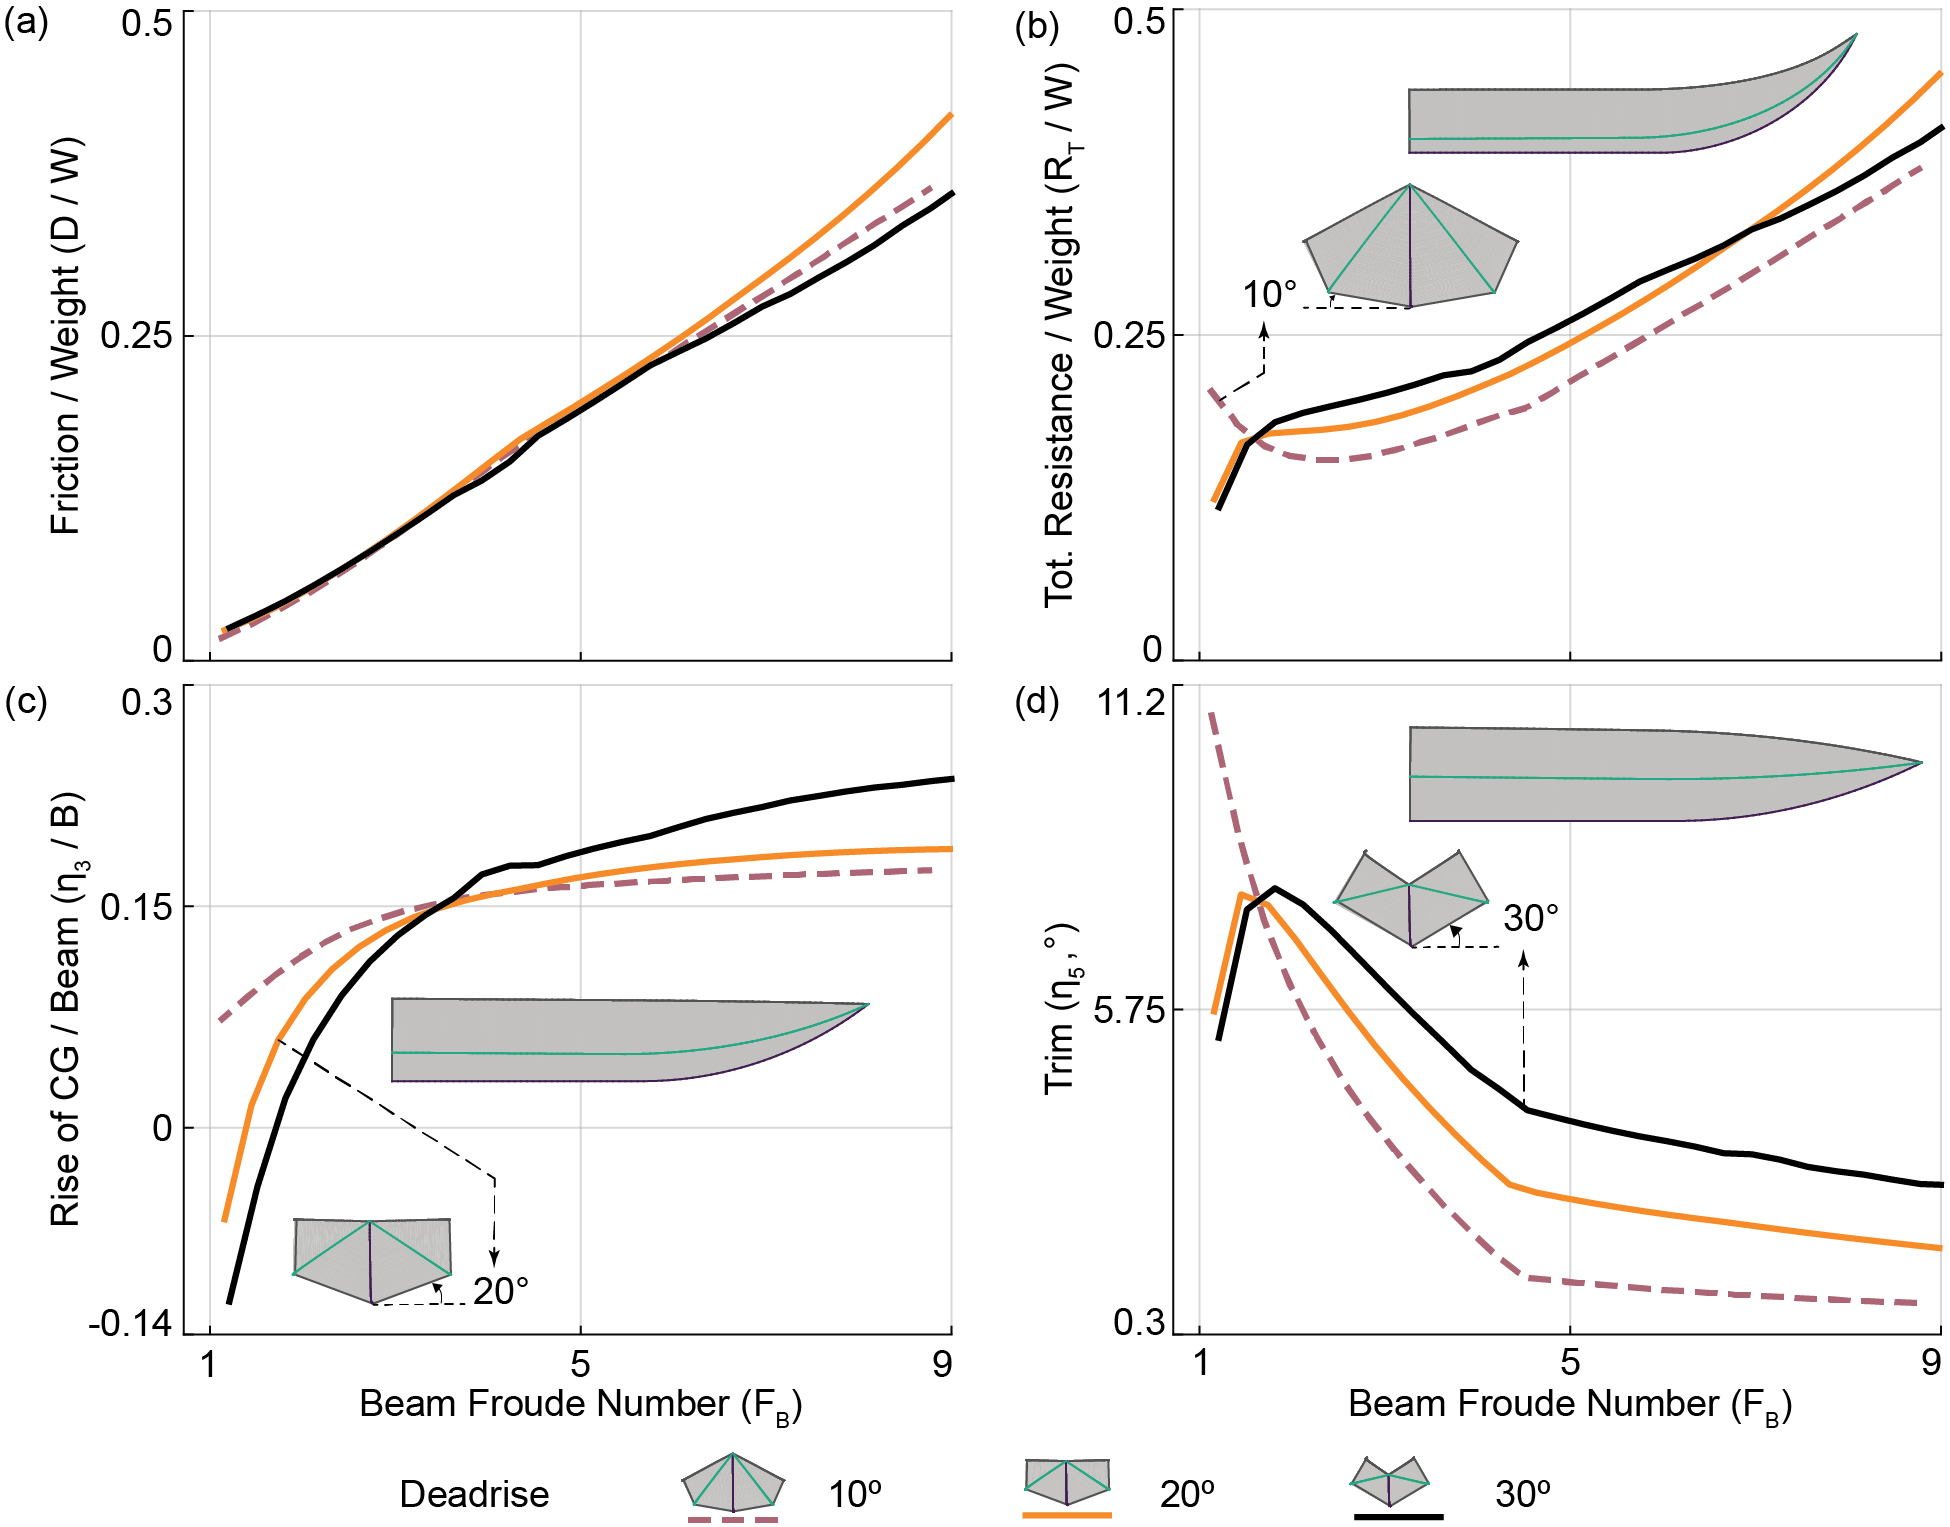
\includegraphics[width=\textwidth]{01-figures/05-06-tunable-calm-hydrodynamics.jpg}
  \caption[]{Effect of varying the CCO hull's deadrise on hydrodynamic performance in calm water: (a) Weight normalized friction drag; (b) Weight normalized total resistance; (c) Beam normalized rise of CG; (d) Trim angle (positive bow up).}
  \label{fig-calm-hydro}
\end{figure}

The influence of shape change on the weight-normalized friction drag experienced by the hull across all deadrise variations is insignificant, except at very high speeds. As illustrated in Fig.~\ref{fig-calm-hydro}\,(a), the 20\(^\circ\) deadrise hull exhibits slightly higher frictional resistance than 10\(^\circ\) and 30\(^\circ\) deadrise configurations at \(F_B\) close to 9. For a lower deadrise configuration, there is an increase in the total resistance at lower speeds, but an interesting reversal of trends emerges at higher speeds. As seen in Fig.~\ref{fig-calm-hydro}\,(b), the lower deadrise configuration now exhibits lower total resistance. A similar trend is also observed for the trim angle of the hull, as shown in Fig.~\ref{fig-calm-hydro}\,(d). This change in trends for total resistance is expected because it is a derived quantity that depends upon the friction drag and trim angle. Since friction drag shows little variation across deadrise configurations, the trend of trim angle contributes to that of the total resistance. In the case of rise of CG, the low deadrise configuration tends to rise higher than the high deadrise configurations for \(F_B\) up to 4, as shown in Fig.~\ref{fig-calm-hydro}\,(c). A noticeable reversal in the hull rise trend emerges at high speeds. The variation in hull rise remains negligible across all deadrise configurations for practical considerations with the exception of the 30\(^\circ\) deadrise configuration. These results can be interpreted in the following ways. In the case of a curved-crease origami hull configured with a lower deadrise, the planing surface typically takes on a flatter and broader profile. Consequently, with increasing surge speed, the hull tends to rise and glide over the water's surface. This phenomenon results in a reduced trim angle as the hull does not have to plow through the water, thereby leading to lower total resistance. In contrast, for a curved-crease origami hull configured with a higher deadrise, the planing surface is generally a shaper V-shape with a narrower profile. This hull tends to sink deeper into the water. Consequently, this hull has to overcome greater total resistance and exhibits increased trim angle at higher surge speeds.

\subsection{Wavy Water Hydrodynamics}\label{05-subsec-wavy-hydro}
The investigation of hull motion in waves is carried out under the condition of a constant speed of 4.04~m/s when navigating head seas. The speed corresponds to \(F_B\) of 2.28, 2.34, and 2.44 for the 10\(^{\circ}\), 20\(^{\circ}\), and 30\(^{\circ}\) deadrise configuration, respectively. Wave amplitudes of 0.02~m are applied to all three hull geometries. Each of the three hull geometries is subjected to regular waves with wavelengths equivalent to 4, 8, and 12 times the overall length of the planing hull. The mean subtracted steady-state hull motion is depicted in Fig.~\ref{fig-wavy-hydro}\,(a-c). These figures display the final 10 seconds of the 100-second time histories and illustrate the heave normalized by wave amplitude and pitch normalized by wave slope of the hulls for the three \(\lambda\)/\(L_{OA}\) ratios.

\begin{figure}[!htbp]
  \centering
  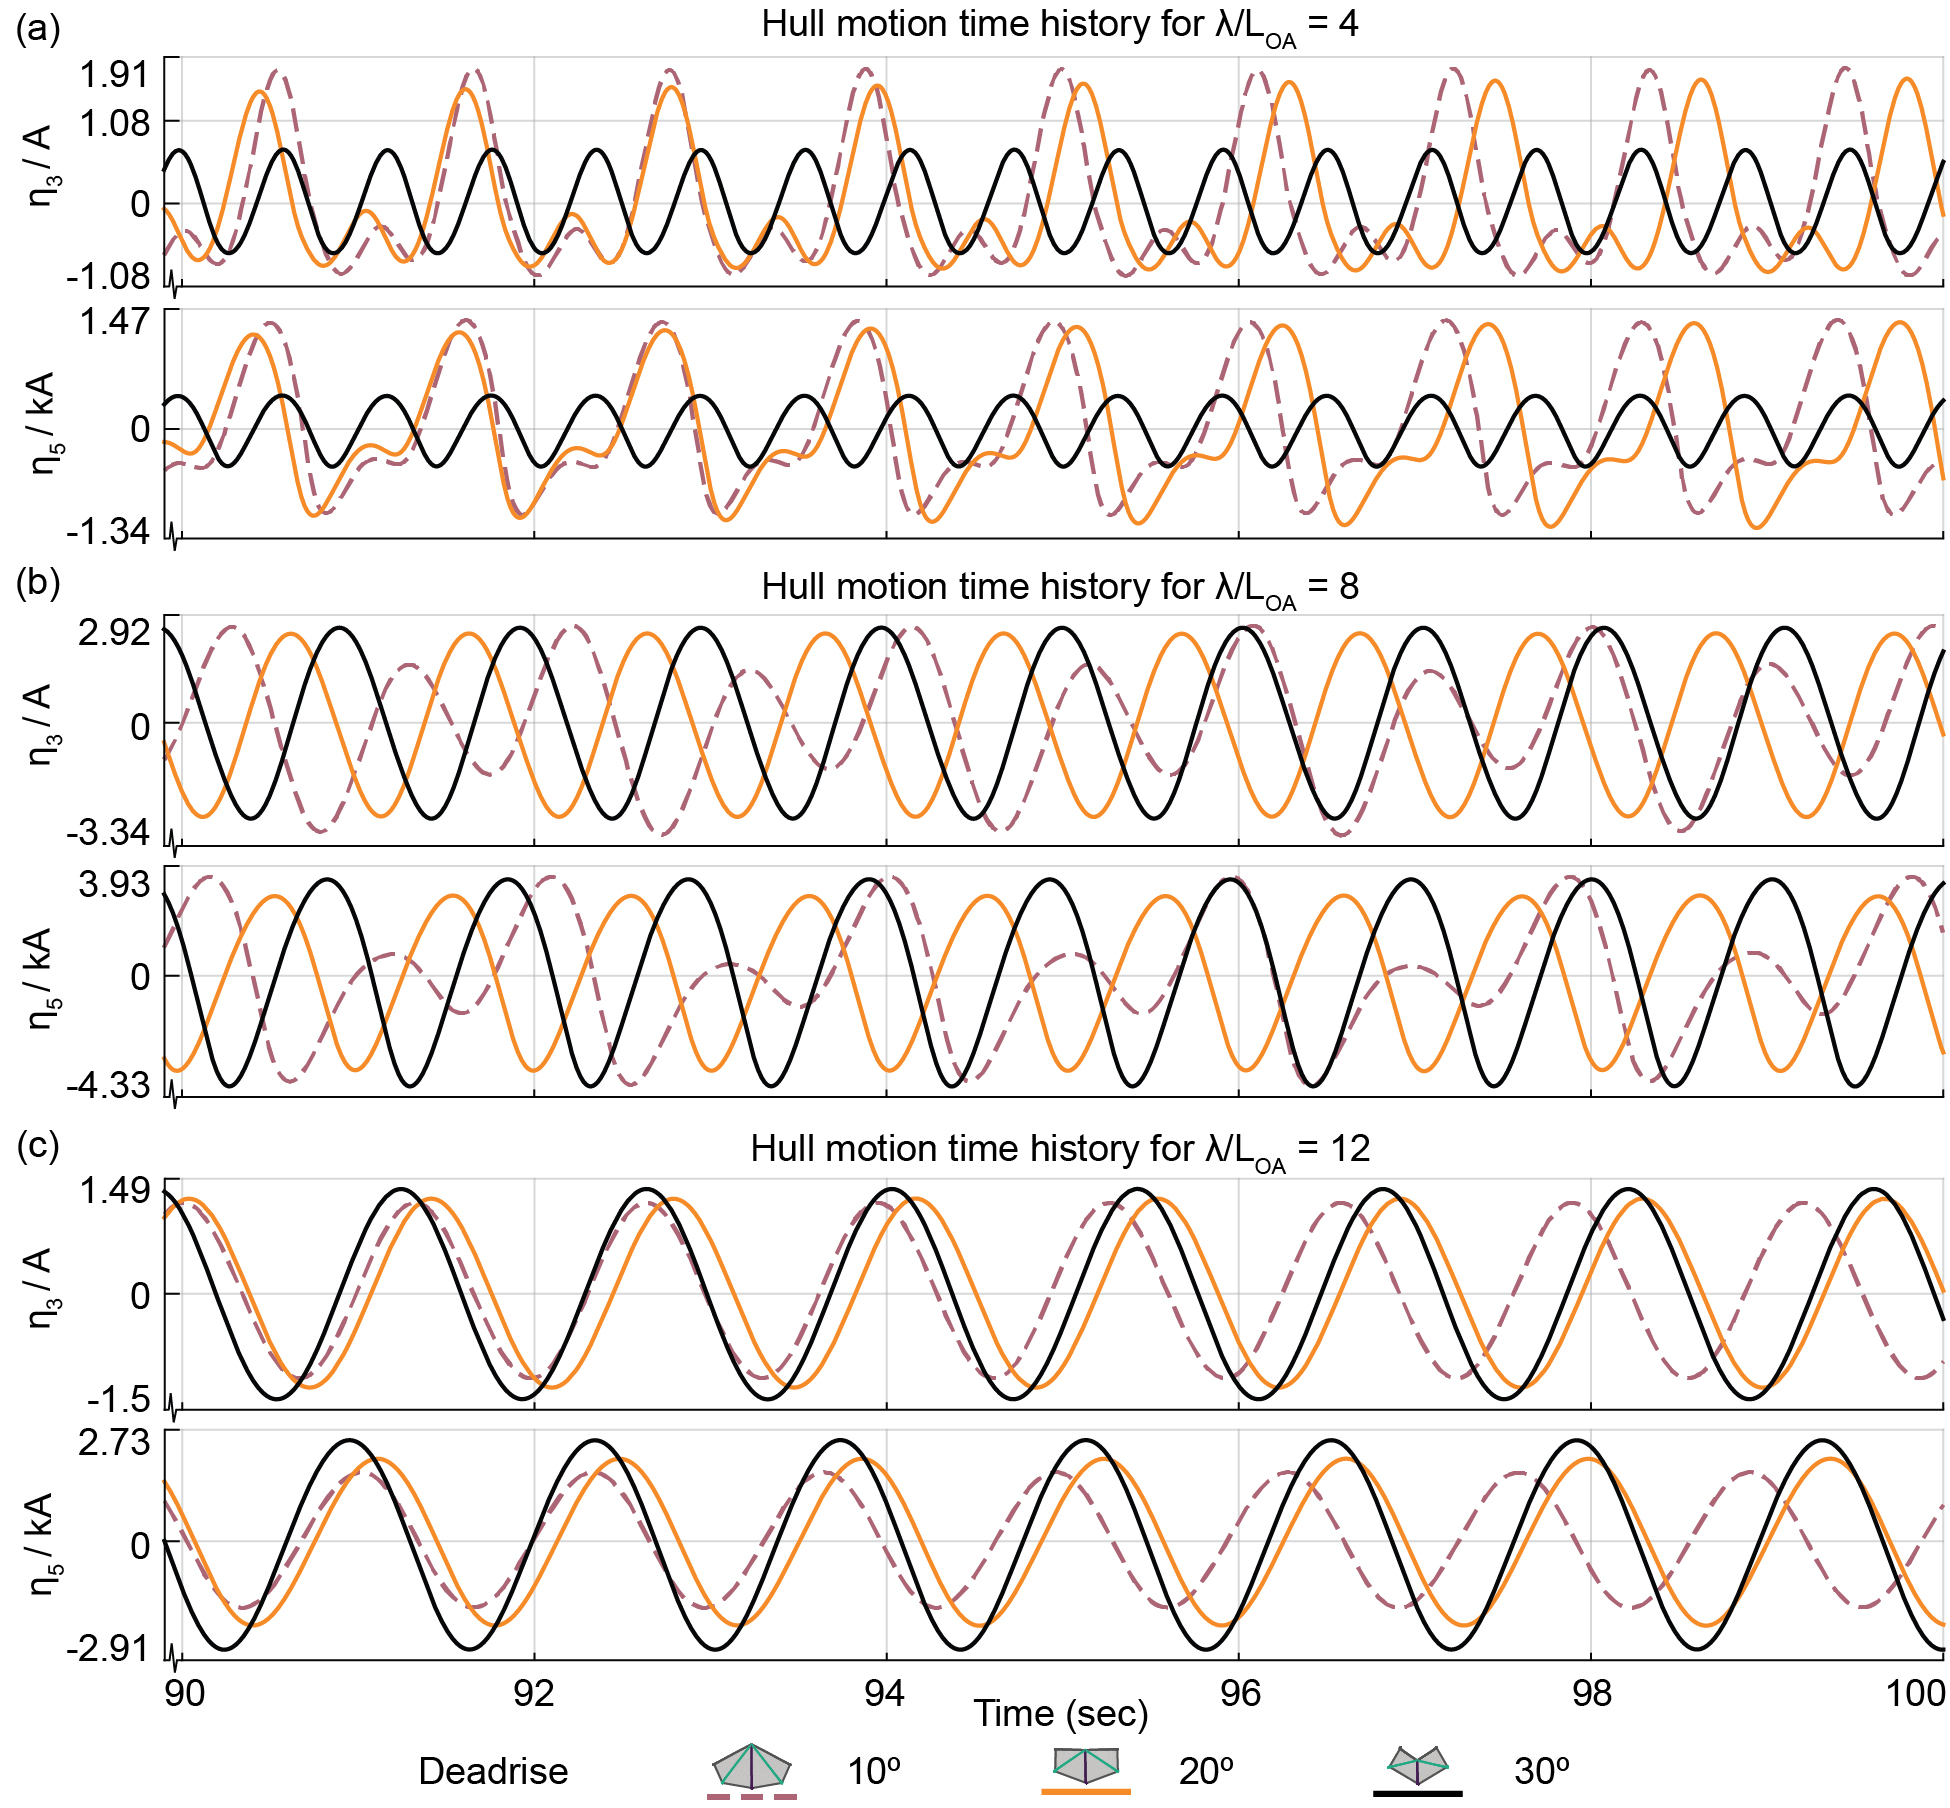
\includegraphics[width=\textwidth]{01-figures/05-07-tunable-wavy-hydrodynamics.jpg}
  \caption{Effect of varying the CCO hull's deadrise on steady state hull motion in head seas for: (a) \(\lambda/L_{OA}\) = 4; (b) \(\lambda/L_{OA}\) = 8; (c) \(\lambda/L_{OA}\) = 12.
  Surge speed is 4.04~m/s, wave amplitude is 0.02~m and the last 10 seconds of the mean subtracted hull motion time history is shown.\,\(\eta_3 / \textrm{A}\) is heave normalized by wave amplitude.\,\(\eta_5 / \textrm{kA}\) is pitch normalized by wave slope.}
  \label{fig-wavy-hydro}
\end{figure}

The objective here is to understand the effects of varying deadrise configurations of the curved-crease origami hull on its performance under different wavy conditions. We observe that the hull configured with 30\(^\circ\) deadrise exhibits strikingly smaller heave and pitch amplitudes for the \(\lambda\)/\(L_{OA}\) ratio of 4 compared to other configurations. As the \(\lambda\)/\(L_{OA}\) ratio increases to 8, the heave and pitch amplitudes increase for all hull shapes. Next, at \(\lambda\)/\(L_{OA}\) ratio of 12, there is a decrease in the motion amplitudes. The hull configured with 10\(^\circ\) deadrise exhibits non-monochromatic hull motion, with higher amplitudes at shorter wavelengths, but reduces in amplitude and becomes monochromatic as the exciting wavelength increases. This hull shape has substantially higher amplitudes at shorter wave frequencies (i.e.~\(\lambda\)/\(L_{OA}\) = 4), which can be expected for planing hulls with lower deadrise angles (flatter hull surface). Our observation here underscores the profound implications of altering the curved-crease origami hull's deadrise configuration on hull motion and overall hydrodynamics. Consequently, the shape-morphing ability of the hull can be harnessed to tune the hull response on-demand, making a single hull geometry adaptable to a wide range of sea conditions.

\section{Physical Implementation}\label{05-sec-physical-implementation}
Translating these designs into practical, life-sized vessels offers several challenges. Critical consideration must be given to selecting appropriate materials for the panels and the flexible joints to ensure the hull's durability while meeting the demands of the naval industry. A preliminary examination of sheet curvature was conducted to identify suitable material options for curved origami panels. Deforming an initially flat sheet to conform to the curved-crease geometry generates significant bending stresses in the sheet itself. These bending stresses can be used to compute a maximum allowable thickness for the sheet, below which the material would remain elastic. The following formula was used to determine the maximum allowable sheet thickness for a given material to fabricate a curved crease origami hull: \( t = 2 \sigma_y / E \kappa \). Here, \(t\) represents the maximum sheet thickness, \(\sigma_y\) corresponds to the material's yield strength, \(E\) denotes the material's Young's modulus, and \(\kappa\) signifies the maximum sheet curvature, obtained from the Bar and Hinge model for a given length of the curved-crease origami hull. Fig.~\ref{fig-prototype}\,(a) graphically depicts the maximum permissible sheet thickness for various materials, such as Aluminium, Glass fiber-reinforced polymer (GFRP), Polycarbonate, Acrylic, and Polyetherimide (Ultem\textregistered{}). This analysis, thus, serves as a crucial reference point for material selection and design considerations in fabricating the curved-crease origami hull.

\begin{figure}[!htbp]
  \centering
  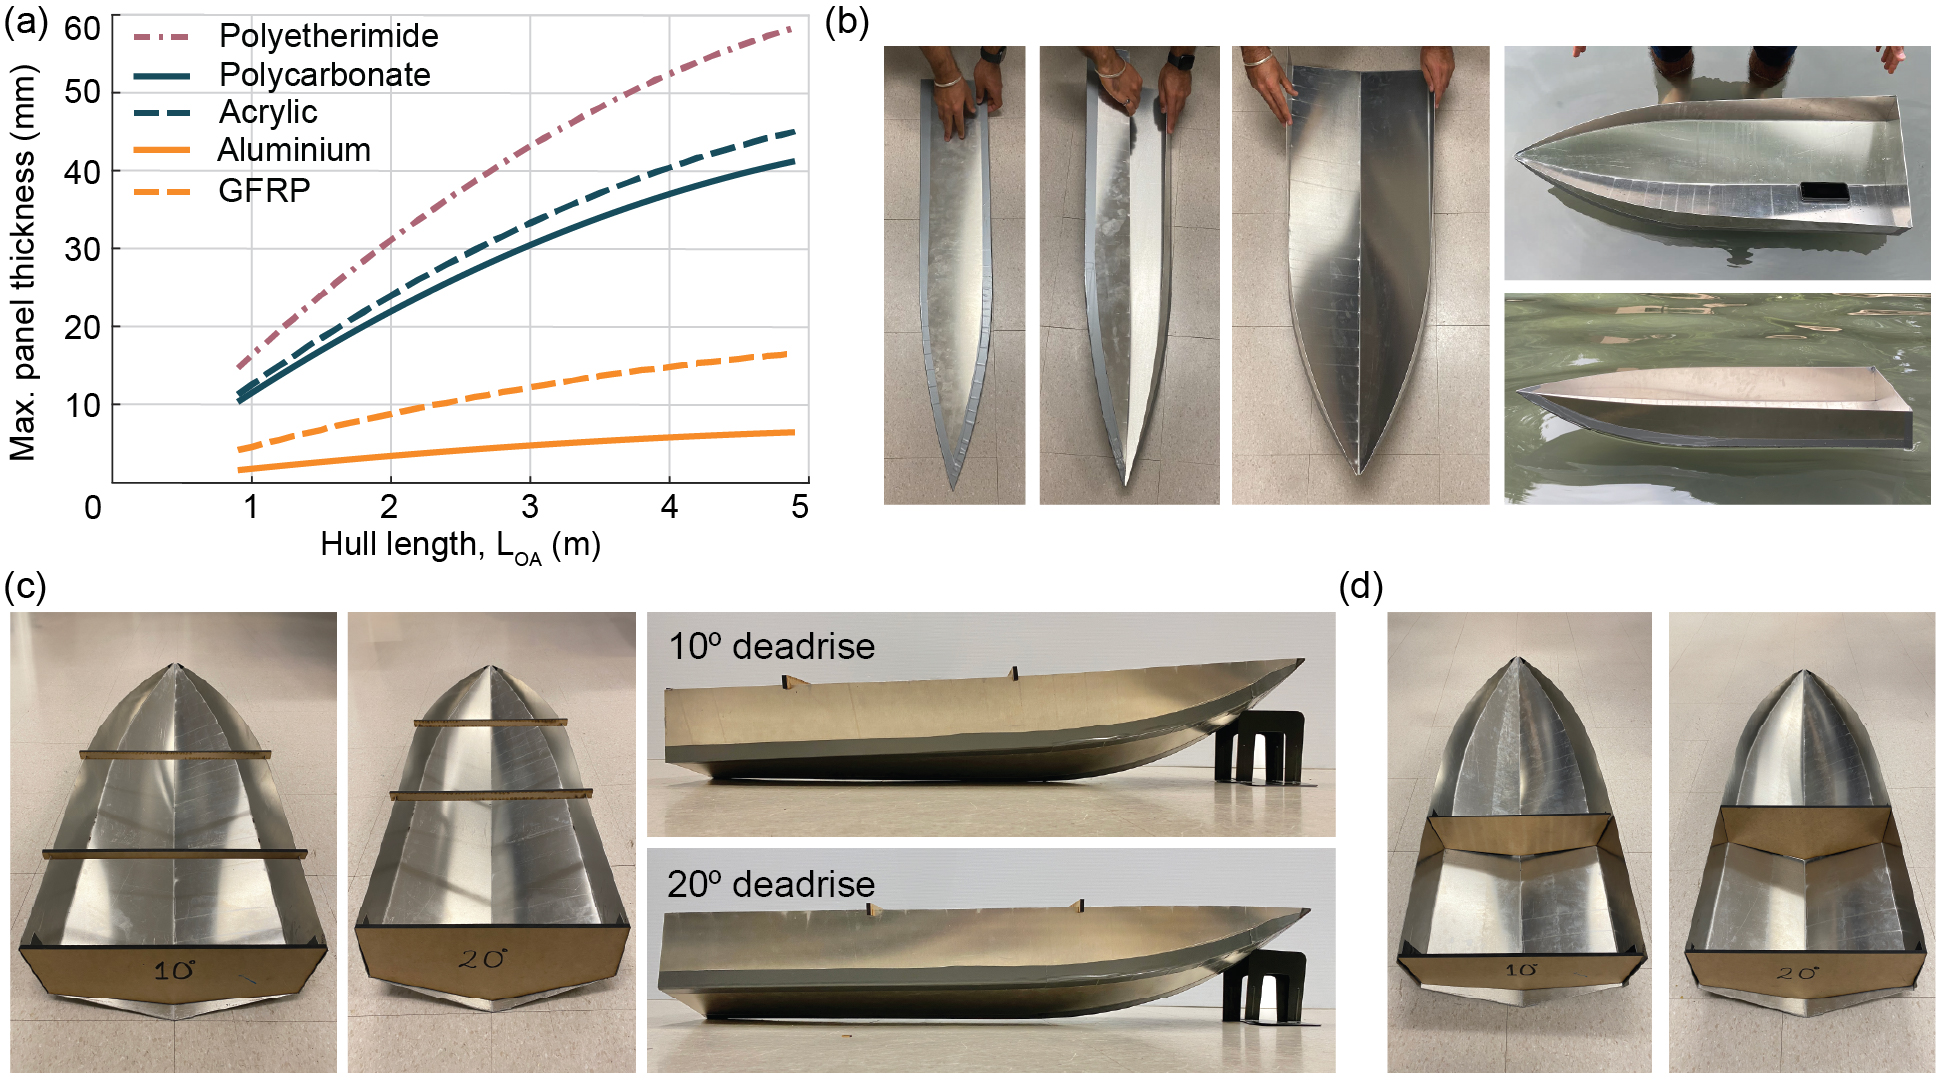
\includegraphics[width=\textwidth]{01-figures/05-08-prototype-scaling-up.jpg}
  \caption{(a) Scalability analysis demonstrating the elastic limit (maximum thickness) for curved-crease origami hulls for different materials; (b) A 91~cm (36~in.) long curved-crease origami hull prototype fabricated using 1.5~mm thick aluminium sheets, joined together with duct tape for flexible joints \textemdash{} displaying the stowed (left) to deployed (right) configuration; (c) Aluminium CCO hull configured with deadrise configurations 10\(^\circ\) and 20\(^\circ\) strengthened with lateral stiffeners that snap onto the side of the hull; (d) Aluminium CCO hulls fitted with solid bulkhead.}
  \label{fig-prototype}
\end{figure}

A scaled model of the curved-crease origami planing hull is constructed by leveraging the results of the curvature analysis. Figure~\ref{fig-prototype}\,(b) showcases a 91~cm (36~inch) long prototype afloat in a water pond, with a smartphone serving as a reference scale. This prototype is constructed using 1.5-millimeter-thick panels of 6061-grade aluminium. The aluminium panels are connected using heavy-duty duct tape along the curved creases, thus serving as the curved-origami fold joints. This prototype serves as an initial proof-of-concept demonstrating the material selection for prototypes to remain elastic. While simplistic, the joints of our prototype are watertight and allow for multiple fold-unfold cycles without degradation.

Post-deployment, the curved crease origami hulls require reinforcement to prevent collapse and torsional deformations. In Fig.~\ref{fig-prototype}\,(c), we present the same aluminium CCO hull from Fig.~\ref{fig-prototype}\,(b), but configured with two distinct deadrise angles \textemdash{} 10\(^\circ\) and 20\(^\circ\). Each deadrise configuration is fortified with snap-fit lateral stiffeners, or girders, constructed from a mid-density fibreboard. These stiffeners effectively prevent collapse and provide sufficient reinforcement against torsional deformations, working in conjunction with the stiffness provided by the transom and curved aluminium sheets. The CCO hulls can also be fitted with solid bulkheads, as shown in Fig.~\ref{fig-prototype}\,(d). In the future, the curved-crease origami hulls can be fitted with deployable bulkheads and stiffeners to strengthen the hull post-deployment.

A parallel fabrication effort was led by Jason P. Kelly and Daniel C. Hart at the Naval Surface Warfare Center, Carderock Division (NSWCCD) for a desktop-scale curved-crease origami-based planing hull~\cite{kelly2025desktop}. This fabrication effort focused on the use of commonly available marine-composite material for the panels and flexible fiber-reinforced neoprene rubber for the curved folds to create an 18~in long prototype of an origami planing hull.

\section{Concluding Remarks}\label{05-sec-hull-conclusion}
This chapter introduces a hull fabrication approach based on curved-crease origami (CCO) principles. Employing the Bar and Hinge model for curved-origami folding and the Hausdorff distance metric, we explored the ability of two CCO hull variants to conform to conventional VPS and GPPH hull shapes. Obtaining conforming designs was achieved by optimizing the geometric parameters of the curved-crease pattern. Next, we demonstrated the ability of CCO hulls to emulate the hydrodynamic performance of conventional hull forms in still and wavy water conditions using the Powersea tool. Finally, we explored the shape-morphing ability of CCO hulls, which enables on-demand tunability of hydrodynamic performance to suit diverse sea conditions. Proof-of-concept prototypes are fabricated to demonstrate the feasibility of CCO for creating hulls.